\chapter{Solution}
\label{cha:solution}

\sloppy

This chapter will present the \texttt{xmlet} solution, its different components and how they interact between them. Generating a Java \textit{fluent interface} based on a \ac{XSD} file includes two distinct tasks:

\begin{enumerate}
\item Parsing the information from the \ac{XSD} file;
\item Generating the \textit{fluent interface} classes based on the resulting information of the previous task.
\end{enumerate}

\noindent
Those tasks are encompassed by two different projects, \hyperref[sec:xsdparser]{XsdParser} and \hyperref[sec:xsdasm]{XsdAsm}. In this case the XsdAsm has a dependency to XsdParser.

\section{XsdParser} % (fold)
\label{sec:xsdparser}

XsdParser is a library that parses a \ac{XSD} file into a list of Java objects. Each different \ac{XSD} tag has a corresponding Java class and the  attributes of a given \ac{XSD} type are represented as fields in Java. All these classes derive from the same abstract class, \texttt{XsdAbstractElement}. All Java representations of the \ac{XSD} elements follow the schema definition for \ac{XSD} elements, referred in Section \ref{sec:xsd}. For example, the \texttt{xsd:annotation} tag only allows \texttt{xsd:appinfo} and \texttt{xsd:documentation} as children nodes, and can also have an attribute named \texttt{id}, therefore XsdParser has the following class as shown in Listing \ref{lst:xsdannotationexample}.

\bigskip

\lstset{language=java, morekeywords={XsdAppInfo, XsdDocumentation, ArrayList, List, XsdIdentifierElements, Document, parse, getFirstChild, getChildNodes, NodeList, DocumentBuilderFactory, DocumentBuilder, newInstance, newDocumentBuilder, String}}

\begin{minipage}{\linewidth}
\begin{lstlisting}[caption={Simplified Version of the Generated XsdAnnotation Class}, label={lst:xsdannotationexample}]
public class XsdAnnotation extends XsdAbstractElement {

    private String id;
    private List<XsdAppInfo> appInfoList = new ArrayList<>();
    private List<XsdDocumentation> documentations = new ArrayList<>();
    
    // (...)
}
\end{lstlisting}
\end{minipage}

\subsection{Parsing Strategy}
\label{sec:parsingstrategy}

The first step of this library is handling the \ac{XSD} file. The Java language has no built in library that parses \ac{XSD} files, so we needed to look for other options. The main libraries found that address this problem were \ac{DOM} and \ac{SAX}. After evaluating the pros and cons of those libraries the choice ended up being \ac{DOM}, since a \ac{XSD} file is a tree of \ac{XML} elements. This choice was based mostly on the fact that \ac{SAX} is an event driven parser and \ac{DOM} is a tree based parser, which is more adequate for the present issue. \ac{DOM} is a library that maps \ac{HTML}, \ac{XHTML} and \ac{XML} files into a tree structure composed by multiple elements, also named nodes. This is exactly what XsdParser requires to obtain all the information from the \ac{XSD} files, which is described in \ac{XML}. 

\noindent
This means that XsdParser uses \ac{DOM} to parse the \ac{XSD} file and obtain its root element, a \texttt{xs:schema} node, performing a single read on the \ac{XSD} file, avoiding multiple reads which are less efficient (Listing \ref{lst:nodelist}). 

\bigskip

\lstset{language=java, morekeywords={Document, parse, getFirstChild, getChildNodes, NodeList, DocumentBuilderFactory, DocumentBuilder, newInstance, newDocumentBuilder, IOException, SAXException, ParserConfigurationException, Node, String}}

\begin{minipage}{\linewidth}
\begin{lstlisting}[caption={DOM Document Parsing}, label={lst:nodelist}]
private Node getSchemaNode(String filePath) 
    throws IOException, SAXException, ParserConfigurationException {
    DocumentBuilderFactory dbFactory =                                                              
                                DocumentBuilderFactory.newInstance();
    DocumentBuilder dBuilder = dbFactory.newDocumentBuilder();
    Document doc = dBuilder.parse(xsdFile);   //Parses the XSD file.

    //Obtains the first node, which is the xs:schema node.
    return doc.getFirstChild();
}
\end{lstlisting}
\end{minipage}

\newpage

\noindent
After obtaining the root node of the \ac{XSD} file the XsdParser verifies if that node is a \texttt{XsdSchema} node as shown in Listing \ref{lst:nodeparsingprocess}. If that is the case it proceeds by performing the \texttt{parse} function of the \texttt{XsdSchema} class.  

\bigskip

\lstset{language=Java, morekeywords={stream, filter, map, forEach, apply, add, getNodeType, getNodeName, get, Node, getSchemaNode, isXsdSchema, XsdSchema, parse}}

\begin{minipage}{\linewidth}
\begin{lstlisting}[caption={XsdParser Parsing the XsdSchema Node which triggers the parsing of the whole XSD document},captionpos=b,label={lst:nodeparsingprocess}]
Node schemaNode = getSchemaNode(filePath);
            
if (isXsdSchema(schemaNode)){
    XsdSchema.parse(this, schemaNode);
}
\end{lstlisting}
\end{minipage}

\noindent
The \texttt{XsdSchema} element \texttt{parse} function converts the \texttt{Node} attributes into a \texttt{Map} object, which \texttt{XsdSchema} receives in the constructor. Each class extracts their field information from that \texttt{Map} object in their \texttt{setFields} method (Listing \ref{lst:xsdschemaparsing}). To guarantee that the information parsed by the classes is valid according to the rules in the \ac{XSD} language standard there are multiple validations. To validate the possible values for any given attribute, e.g. the \texttt{formDefault} attribute from the \texttt{xsd:schema} element, we use \texttt{Enum} classes. Any parsed value that is meant to be assigned to one of this \texttt{Enum} variables has its content verified to assert if the received value belongs to the possible values for that attribute. 

\bigskip

\lstset{language=Java, morekeywords={getOrDefault, NamedNodeMap, Map, String, getAttributes, convertNodeMap, XsdSchema, XsdParser, ELEMENT_FORM_DEFAULT, ATTRIBUTE_FORM_DEFAULT, BLOCK_DEFAULT, FINAL_DEFAULT, TARGET_NAMESPACE, VERSION, XMLNS, @Override, XsdAnnotatedElements, EnumUtils, belongsToEnum, FormEnum, UNQUALIFIED, getValue, DEFAULT, BlockFinalEnum, FinalDefaultEnum, Node}}

\begin{lstlisting}[caption={XsdSchema Extracting Information from the received Node},captionpos=b,label={lst:xsdschemaparsing}]
public class XsdSchema extends XsdAnnotatedElements {
    private XsdSchema(XsdParser parser, Map<String, String> fieldsMap){
        super(parser, fieldsMap);
    }
    
    @Override
    public void setFields(Map<String, String> fieldsMap) {
        super.setFields(fieldsMap);

        this.attributeFormDefault = 
        	AttributeValidations.belongsToEnum(FormEnum.UNQUALIFIED, 				
        		elementFieldsMap.getOrDefault(ATTRIBUTE_FORM_DEFAULT, 
        			FormEnum.UNQUALIFIED.getValue()));
        this.elementFormDefault = 			 
        	AttributeValidations.belongsToEnum(FormEnum.UNQUALIFIED, 		
        		elementFieldsMap.getOrDefault(ELEMENT_FORM_DEFAULT, 	
        			FormEnum.UNQUALIFIED.getValue()));
        this.blockDefault = 		
            AttributeValidations.belongsToEnum(BlockFinalEnum.DEFAULT, 		
        		elementFieldsMap.getOrDefault(BLOCK_DEFAULT, 	
        			BlockFinalEnum.DEFAULT.getValue()));
        this.finalDefault = 
            AttributeValidations.belongsToEnum(FinalDefaultEnum.DEFAULT, 
        		elementFieldsMap.getOrDefault(FINAL_DEFAULT, 
        			FinalDefaultEnum.DEFAULT.getValue()));
        this.targetNamespace = 
        	elementFieldsMap.getOrDefault(TARGET_NAMESPACE, targetNamespace);
        this.version = elementFieldsMap.getOrDefault(VERSION, version);
        this.xmlns = elementFieldsMap.getOrDefault(XMLNS, xmlns);
    }
    
    public static ReferenceBase parse(XsdParser parser, Node node) {
        NamedNodeMap nodeAttributes = node.getAttributes();
        Map<String, String> attrMap = convertNodeMap(nodeAttributes);        
    
        return xsdParseSkeleton(node, new XsdSchema(parser, attrMap));
    }
}
\end{lstlisting}

\noindent
The parsing of the \texttt{XsdSchema} continues by parsing its children nodes. To parse children elements of any given \texttt{XsdAbstractElement} type we have the \texttt{xsdParseSkeleton} function present in the \texttt{XsdAbstractElement} class (Listing \ref{lst:skeletonfunction}). This function will iterate in all the children of a given node, invoke the respective \texttt{parse} function of each children and then notify the parent element, using the Visitor pattern\cite{gamma1994design}. 

\noindent
In the XsdParser the Visitor pattern is used to ensure that each concrete element defines different behaviours for different types of children. This provides good flexibility for implementing certain \ac{XSD} syntax restrictions, e.g. the element A can reject the element B as his children if the element A does not support children of type B.

\noindent
By using this strategy we ensure that the whole \ac{XSD} file is parsed just by invoking the \texttt{parse} function of \texttt{XsdSchema}. This happens because the \texttt{XsdSchema} element is the top level element of all the \ac{XSD} files and having all the concrete element types parsing their children will result in the parsing of the whole \ac{XSD} file.

\bigskip

\lstset{language=Java, morekeywords={Node, XsdAbstractElement, getFirstChild, getNodeType, getNodeName, String, Function, getParseMappers, get, apply, getElement, accept, getVisitor, getNextSibling, createFromXsd, ReferenceBase, XsdParser, getParser, ELEMENT_NODE, BiFunction, XsdParser, addParsedElement}}

\begin{minipage}{\linewidth}
\begin{lstlisting}[caption={XsdParseSkeleton Function - Parsing Children From a Node},captionpos=b,label={lst:skeletonfunction}]
ReferenceBase xsdParseSkeleton(Node node, XsdAbstractElement element){
    XsdParser parser = element.getParser();
    Node child = node.getFirstChild();

    while (child != null) { //Iterates in all children from node.
        //Only parses element nodes, ignoring comments and text nodes.
        if (child.getNodeType() == Node.ELEMENT_NODE) { 
            String nodeName = child.getNodeName();

            //Searches on a mapper for a parsing functions 
            //for the respective type.
            BiFunction<XsdParser, Node, ReferenceBase> parserFunction = XsdParser.getParseMappers().get(nodeName);

            //Applies the parsing functions, if any, and notifies 
            //the parent objects Visitor to the newly created object.
            if (parserFunction != null){
                XsdAbstractElement childElement =
                	parserFunction.apply(parser, child).getElement();
                
                childElement.accept(element.getVisitor());
                childElement.validateSchemaRules();
            }
        }

        child = child.getNextSibling(); //Moves on to the next sibling.
    }

    ReferenceBase wrappedElement= ReferenceBase.createFromXsd(element);
    parser.addParsedElement(wrappedElement);
    return wrappedElement;
}
\end{lstlisting}
\end{minipage}

\noindent
Based on the explanation provided above, we will give a more detailed description about the parsing process made by \texttt{XsdParser} using a small concrete example extracted from the \ac{HTML} \ac{XSD} file, present in Listing \ref{lst:parsingexample}.

\bigskip

\lstset{
	language=XML,
	morekeywords={xs:schema, xmlns, targetNamespace, xmlns:xs, name, xs:element, xs:complexType, id}
}

\begin{minipage}{\linewidth}
\begin{lstlisting}[caption={Parsing Concrete Example},captionpos=b,label={lst:parsingexample}]
<xs:schema>
    <xs:element name="html">
        <xs:complexType>
            <!-- -->
        </xs:complexType>
    </xs:element>
</xs:schema>
\end{lstlisting}
\end{minipage}


Step 1 - DOM parsing:

\noindent
The parsing starts with the \ac{DOM} library parsing the code (Listing \ref{lst:parsingexample}), which returns the \texttt{xs:schema} node (i.e. schemaNode in Listing \ref{lst:nodeparsingprocess}). \texttt{XsdParser} verifies if the node is in fact a \texttt{xs:schema} node and after verifying that in fact it is, it invokes the \texttt{XsdSchema parse} function (line 19 of Listing \ref{lst:xsdschemaparsing}). 

Step 2 - XsdSchema Attribute Parsing:

\noindent
The \texttt{XsdSchema parse} function receives the \texttt{Node} object and converts it to a \texttt{Map} object (line 21 of Listing \ref{lst:xsdschemaparsing}). The map object is then passed to the \texttt{XsdSchema} constructor which will result in the invocation of the \texttt{setFields} method (line 7 of Listing \ref{lst:xsdschemaparsing}), which will extract the information from the \texttt{Map} object to the class fields.

Step 3 - XsdSchema Children:

\noindent
To parse the \texttt{XsdSchema} children the \texttt{XsdAbstractElement xsdParseSkeleton} (Listing \ref{lst:skeletonfunction}) function is called (line 24 of Listing \ref{lst:xsdschemaparsing}) and starts to iterate the \texttt{xs:schema} node children, which, in this case, is a node list containing a single element, the \texttt{xs:element} node. 

Step 4 - XsdElement Attribute Parsing:

\noindent
The parsing of the \texttt{xs:element} node is similar to \texttt{xs:schema}, it extracts the attribute information from its respective node in its \texttt{setFields} function. 

Step 5 - XsdSchema Visitor Notification:

\noindent
After parsing the \texttt{xs:element} node the previously created \texttt{XsdSchema} object is notified using the Visitor pattern. This notification informs the \texttt{XsdSchema} object that it contains the newly created \texttt{XsdElement} object. The \texttt{XsdSchema} should then act accordingly based on the type of the object received as his children, since different types of objects should be treated differently.

\subsection{Reference solving}
\label{sec:refsolving}

After the parsing process described previously, there is still an issue to solve regarding the existing references in the \ac{XSD} schema definition. In \ac{XSD} files the usage of the \texttt{ref} attribute is frequent to avoid repetition of \ac{XML} code. This generates two main problems when handling reference solving, the first one being existing elements with \texttt{ref} attributes referencing non existent elements and the other being the replacement of the reference object by the referenced object when present. In order to effectively help resolve the referencing problem some wrapper classes were added. These wrapper classes contain the wrapped element and serve as a classifier for the wrapped element. The existing wrapper classes are as follow:

\begin{itemize}  
	\item \texttt{UnsolvedElement} - Wrapper class to each element that has a \texttt{ref} attribute.
	\item \texttt{ConcreteElement} - Wrapper class to each element that is present in the file.
	\item \texttt{NamedConcreteElement} - Wrapper class to each element that is present in the file and has a \texttt{name} attribute present.
	\item \texttt{ReferenceBase} - A common interface between \texttt{UnsolvedReference} and \texttt{ConcreteElement}.
\end{itemize}

\noindent
Having these wrappers on the elements allow for a detailed filtering, which is helpful in the reference solving process. That process starts by obtaining all the \texttt{NamedConcreteElement} objects since they may or may not be referenced by an existing \texttt{UnsolvedReference} object. The second step is to obtain all the \texttt{UnsolvedReference} objects and iterate them to perform a lookup search on the \texttt{NamedConcreteElement} objects obtained previously. This is achieved by comparing the value present in the \texttt{UnsolvedReference ref} attribute with the \texttt{NamedConcreteElement name} attribute. If a match is found then XsdParser performs a copy of the object wrapped by the \texttt{NamedConcreteElement} and replaces the element wrapped in the \texttt{UnsolvedReference} object that served as a placeholder. A concrete example of how this process works is in Listing \ref{lst:refsolvingexample}.

\bigskip

\lstset{language=XML, morekeywords={encoding, xsd:schema, xmlns, xmlns:xsd, xsd:group, xsd:choice, id, name,  ref}}

\begin{minipage}{\linewidth}
\begin{lstlisting}[caption={Reference Solving Example},captionpos=b,label={lst:refsolvingexample}]
<xsd:schema xmlns='http://schemas.microsoft.com/intellisense/html-5' xmlns:xsd='http://www.w3.org/2001/XMLSchema'>
	
    <!-- NamedConcreteType wrapping a XsdGroup -->
    <xsd:group id="replacement" name="flowContent">
				<!-- (...) -->
    </xsd:group>
	
    <!-- ConcreteElement wrapping a XsdChoice -->
    <xsd:choice>
        <!-- UnsolvedReference wrapping a XsdGroup -->
        <xsd:group id="toBeReplaced" ref="flowContent"/>
    </xsd:choice>
</xsd:schema>
\end{lstlisting}
\end{minipage}

\noindent
In this short example we have a \texttt{XsdChoice} element that contains a \texttt{XsdGroup} element with a \texttt{ref} attribute. When replacing the \texttt{UnsolvedReference} objects the \texttt{XsdGroup} with the \texttt{ref} attribute is going to be replaced by a copy of the already parsed \texttt{XsdGroup} with the \texttt{name} attribute. This is achieved by accessing the parent of the element, in this case accessing the parent of the \texttt{XsdGroup} with the \texttt{ref} attribute, in order to remove the element identified by "toBeReplaced" and adding the element identified by "replacement".

\noindent
Having created these classes it is expected that at the end of a successful file parsing only \texttt{ConcreteElement} and/or \texttt{NamedConcreteElement} objects remain. In case there are any remainder \texttt{UnsolvedReference} objects the programmer can query the parser, using the function \texttt{getUnsolvedReferences} of the \texttt{XsdParser} class, to discover which elements are missing and where were they used. The programmer can then correct the missing elements by adding them to the \ac{XSD} file and repeat the parsing process or just acknowledge that those elements are missing. 

\subsection{Validations}

As it was already referred in Section \ref{sec:parsingstrategy} the parser uses some strategies to validate the rules of the \ac{XSD} language. We already referred the usage of \texttt{Enum} classes for attribute values that have a set of possible values but there are more validations. This solution also validates the types of data received, e.g. validating if a given attribute is a positive \texttt{Integer} value. There are other more intricate restrictions relating to the organization between elements, for example the \texttt{xsd:element} element is not allowed to have a \texttt{ref} attribute value if the \texttt{xsd:element} is a direct child of the top-level \texttt{xsd:schema} element. All those rules were extracted from the \ac{XSD} language standard and each time a concrete element is create the respective rules are verified as seen with the \texttt{validateSchemaRules} method call in line 21 of Listing \ref{lst:skeletonfunction}. 

\noindent
Each time any of these rules are violated a \texttt{ParsingException} is thrown containing a message detailing the rule that was violated, either being an attribute that does not match its type, an attribute that has a value that is not within the possible values for that attribute or the other more complex rules of the \ac{XSD} language. With this strategy the user of the XsdParser solution has the information needed to fix the existing problems in the \ac{XSD} file.

\section{XsdAsm} % (fold)
\label{sec:xsdasm}

XsdAsm is a library dedicated to generate a Java \textit{fluent interface} based on a \ac{XSD} file. It uses the previously introduced XsdParser library to parse the \ac{XSD} file contents into a list of Java elements that XsdAsm will use to obtain the information needed to generate the correspondent classes. 

\noindent
To generate classes this library also uses the ASM\cite{asm} library, which is a library that provides a Java interface that allows \textit{bytecode} manipulation providing methods for creating classes, methods, etc. There were other alternatives to the ASM library but most of them are simply libraries that were built on top of ASM to simplify its usage. It supports the creation of Java classes up until Java 9 and is still maintained, the most recent version, 6.2.1, was release in 5 August of 2018. ASM also has some tools to help the new programmers understand how the library works. These tools help the programmers to learn faster how the code generation works and allow to increase the complexity of the generated code. In Listing \ref{lst:asmexampleobjective} we present a class that is the objective of our code generation, it is a simple class, with a field and a method. The ASM library provides a tool, \texttt{ASMifier}, that receives a \texttt{.class} file and returns the ASM code needed to generate it, as shown in Listing \ref{lst:asmexamplecode}.

\bigskip

\lstset{language=Java, morekeywords={encoding, xsd:schema, xmlns, xmlns:xsd, xsd:group, xsd:choice, id, name,  ref}}

\begin{minipage}{\linewidth}
\begin{lstlisting}[caption={ASM Example - Code Generation Objective},captionpos=b,label={lst:asmexampleobjective}]
public class SumExample {

    private int sum;

    void setSum(int a, int b){
        sum = a + b;
    }
}
\end{lstlisting}
\end{minipage}

\bigskip

\lstset{language=Java, morekeywords={ClassWriter, visit, V9, ACC_PUBLIC, ACC_FINAL, ACC_SUPER, visitField, ACC_PRIVATE, FieldVisitor, visitEnd, visitMethod, visitCode, visitVarInsn, visitInsn, visitFieldInsn, PUTFIELD, ILOAD, ALOAD, IADD, RETURN, visitMaxs, writeByteArrayToFile, toByteArray}}

\begin{minipage}{\linewidth}
\begin{lstlisting}[caption={ASM Example - Required Code},captionpos=b,label={lst:asmexamplecode}]
ClassWriter classWriter = new ClassWriter(0);

classWriter.visit(V9, ACC_PUBLIC + ACC_FINAL + ACC_SUPER, 
	"Samples/HTML/SumExample", null, "java/lang/Object", null);

FieldVisitor fieldVisitor = 
	classWriter.visitField(ACC_PRIVATE, "sum", "I", null, null);
fieldVisitor.visitEnd();

MethodVisitor methodVisitor = 
	classWriter.visitMethod(0, "setSum", "(II)V", null, null);
methodVisitor.visitCode();
methodVisitor.visitVarInsn(ALOAD, 0);
methodVisitor.visitVarInsn(ILOAD, 1);
methodVisitor.visitVarInsn(ILOAD, 2);
methodVisitor.visitInsn(IADD);
methodVisitor.visitFieldInsn(PUTFIELD, "Samples/HTML/SumExample",
	"sum", "I");
methodVisitor.visitInsn(RETURN);
methodVisitor.visitMaxs(3, 3);
methodVisitor.visitEnd();

classWriter.visitEnd();

writeByteArrayToFile(classWriter.toByteArray());
\end{lstlisting}
\end{minipage}

\noindent
The strategy while creating the \texttt{xmlet} solution was to have manually created classes that represent a certain type of class that XsdASm will need to generate, i.e. the concrete element, attribute classes. By using the \texttt{ASMifier} tool with those template-like classes the programming process was expedited.

\subsection{Supporting Infrastructure}
\label{sec:supportinginfrastructure}

To support the foundations of the \ac{XSD} language an infrastructure is created in every \textit{fluent interface} generated by this project. This infrastructure is composed by a common set of classes. This supporting infrastructure is divided into three different groups of classes:

Element classes:

\begin{itemize}  
	\item \texttt{Element} - An interface that serves as a base to every parsed \ac{XSD} element.
	\item \texttt{AbstractElement} - An abstract class from where all the \ac{XSD} element derive. This class implements most of the methods present on the \texttt{Element} interface.
\end{itemize}

Attribute classes:

\begin{itemize}  
	\item \texttt{Attribute} - An interface that serves as a base to every parsed \ac{XSD} attribute.
	\item \texttt{BaseAttribute} - A class that implements the \texttt{Attribute} interface. 
\end{itemize}

Visitor class:

\begin{itemize}
	\item \texttt{ElementVisitor} - An abstract class that defines methods for all the generated elements that can be visited with the Visitor pattern. All the implemented methods point to a single method. This behaviour aims to reduce the amount of code needed to create concrete implementations of this class.
\end{itemize}

\noindent
Taking in consideration those classes, a very simplistic \textit{fluent interface} could be represented with the class diagram (Figure \ref{img:infrastructure}). In this example we have an element, \texttt{Html}, that extends \texttt{AbstractElement} and an attribute, \texttt{AttrManifestString}, that extends \texttt{BaseAttribute}. 

\begin{figure}[H]
	\centering
	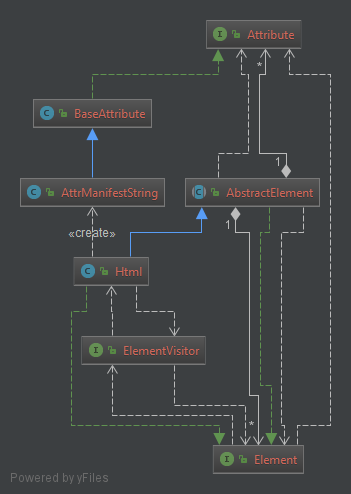
\includegraphics[width=0.8\textwidth]{infrastructure}
	\caption{Fluent Interfaces - The Supporting Infrastructure}
	\label{img:infrastructure}
\end{figure}

\subsection{Code Generation Strategy}
\label{sec:codegenerationstrategy}

As we already presented before in the Section \ref{sec:problemstatement}, this solution focus on how the code is organized instead of making complex code. All the methods present in the generated classes have very low complexity, mainly adding information to the element children and attribute list. To reduce repeated code many interfaces with default methods are created so different classes can implement them and reuse the code. The complexity of the generated code is mostly present in the \texttt{AbstractElement} class, which implements most of the \texttt{Element} interface methods. Another very important aspect of the generated classes is the extensive use of \textit{type arguments} which allows the navigation in the element tree while maintaining type information which is essential to guarantee the specific language restrictions.

\subsection{Type Parameters}
\label{sec:typeparameters}

As this solution was designed an objective became clear, the generated \textit{fluent interface} should be easily navigable. This is crucial to provide a good user experience while creating templates through the \texttt{xmlet} fluent interfaces. There are two main aspects, the fluent interface should be easily navigable and always implement the concrete language restrictions. To tackle this issue we rely on \textit{type arguments}. Through \textit{type parameters} we can always keep track of the tree structure of the elements that are being created and keep adding elements or moving up in the tree structure. In Listing \ref{lst:typeargumentsexplicit} we can observe how the type arguments work. 

\bigskip

\lstset{language=Java, morekeywords={Html, Body, Div, body, div, attrClass, Element}}

\begin{minipage}{\linewidth}
\begin{lstlisting}[caption={Example of the Explicit Use of Type Arguments},captionpos=b,label={lst:typeargumentsexplicit}, literate={º}{\textdegree}1]
Html<Element> html = new Html<>();
Body<Html<Element>> body = html.body();
Div<Body<Html<Element>>> div = body.div();
Div<Body<Html<Element>>> divAfterAttribute = 
                         div.attrClass("attrClassValue");
Body<Html<Element>> bodyAgain = divAfterAttribute.º();
Html<Element> htmlAgain = bodyAgain.º();
\end{lstlisting}
\end{minipage}

\noindent
When we create the \texttt{Html} element we should indicate that he has a parent, for consistency. Then, as we add elements such as \texttt{Body} we automatically return the recently created \texttt{Body} element, but with parent information that indicates that this \texttt{Body} instance is descendant of an \texttt{Html} element. The same happens with the \texttt{Div} element. This behavior changes when adding attributes, in which case we return the object which had the attribute added to them, while maintaining all the parent information. The last two lines show how to move up in the element tree by using the method \texttt{º}. The method name is meant to be as short as possible and to avoid distractions while reading the template. 

\noindent
While in the example presented in Listing \ref{lst:typeargumentsexplicit} the usage of the \textit{fluent interface} might seem to have excessive verbose to define a simple \ac{HTML} document that verbose is not exactly needed. For specific purposes it might be needed to extract variables but the most common usage of the fluent interface should be more similar to Listing \ref{lst:typeargumentshidden}.  

\bigskip

\lstset{language=Java, morekeywords={Html, body, div,attrClass}}

\begin{minipage}{\linewidth}
\begin{lstlisting}[caption={Example of the Implicit Use of Type Arguments},captionpos=b,label={lst:typeargumentshidden}, literate={º}{\textdegree}1]
new Html<>()
      .body()
           .div().attrClass("attrClassValue").º()
      .º();
\end{lstlisting}
\end{minipage}

\noindent
To provide a better understanding on how this is possible we need to showcase three distinct classes. First we have the \texttt{AbstractElement} class, Listing \ref{lst:abstractelement}, from which all concrete elements derive. This class receives two \textit{type parameters}: 

\begin{itemize}
	\item \textbf{T} - Represents the type of the concrete element; 
	\item \textbf{Z} - Represents the type of the parent of the concrete element.
\end{itemize}	

\lstset{language=Java, morekeywords={AbstractElement, Element, T, Z}}

\noindent
In the \texttt{º} method, which returns the parent of any concrete element, the \textit{type parameter} is guaranteed by returning \texttt{Z}, which is the type of the parent of the current element, as shown in the last two lines of code of Listing \ref{lst:typeargumentsexplicit}.

\bigskip

\begin{minipage}{\linewidth}
\begin{lstlisting}[caption={AbstractElement Class Type Arguments},captionpos=b,label={lst:abstractelement}, literate={º}{\textdegree}1]
class AbstractElement<T extends Element, Z extends Element>
	protected Z parent;
	
    protected AbstractElement(Z parent) {
        this.parent = parent;
    }	
	
	public Z º() {
		return this.parent;
	}
	
	// (...)
}
\end{lstlisting}
\end{minipage}

\noindent
The second class is the \texttt{Html} class, which is representative of every concrete element of an \texttt{xmlet} \textit{fluent interface}. It has a single \textit{type parameter}, Z which represents the type of its parent. It extends \texttt{AbstractElement} and therefore indicates that his type is \texttt{Html<Z>} and its parent type is \texttt{Z}. Any  interface implemented by the concrete elements should receive the same type information as the \texttt{AbstractElement} class, as shown with \texttt{HtmlChoice0}. Regarding the \texttt{attrManifest} method, it indicates that returns the exact same instance as the one from which the method is called, keeping the type information by returning \texttt{Html<Z>}.

\bigskip

\lstset{language=Java, morekeywords={Html, Element, Z, AbstractElement, HtmlChoice0, addAttr, AttrManifestString, String}}

\begin{minipage}{\linewidth}
\begin{lstlisting}[caption={Html Class Type Arguments},captionpos=b,label={lst:abstractelement}, literate={º}{\textdegree}1]
class Html<Z extends Element> extends AbstractElement<Html<Z>, Z>
                               implements HtmlChoice0<Html<Z>, Z>
    // (...)
    
    public Html<Z> attrManifest(String attrManifest) {
        return this.addAttr(new AttrManifestString(attrManifest));
    }
}
\end{lstlisting}
\end{minipage}

\noindent
As the third class we have the \texttt{HtmlChoice0} interface which is representative of most interfaces of an \texttt{xmlet} \textit{fluent interface}. It should receive the same \textit{type parameters} as \texttt{AbstractElement}:

\begin{itemize}
	\item \textbf{T} - Represents the type of the concrete element; 
	\item \textbf{Z} - Represents the type of the parent of the concrete element.
\end{itemize}	

\noindent
Since the \texttt{Html} is the only class implementing this interface its \texttt{T} \textit{type argument} is always \texttt{Html<Z>} which results in a return type of \texttt{Body<Html<Z>}\texttt{>} when the method \texttt{body} is called. 

\bigskip

\lstset{language=Java, morekeywords={Html, Element, Z, Body, T, addChild, AbstractElement, HtmlChoice0, addAttr, AttrManifestString, self}}

\begin{minipage}{\linewidth}
\begin{lstlisting}[caption={HtmlChoice0 Interface Type Arguments},captionpos=b,label={lst:abstractelement}, literate={º}{\textdegree}1]
interface HtmlChoice0<T extends Element<T, Z>, Z extends Element> 		                                           extends Element<T, Z> {
    default Body<T> body() {
        return (Body)this.addChild(new Body(this.self()));
    }
}
\end{lstlisting}
\end{minipage}

\subsection{Restriction Validation}
\label{sec:restrictionvalidation}

In the description of any given \ac{XSD} file there are many restrictions in the way the elements are contained in each other and which attributes are allowed. To reflect those restrictions to Java language there are two alternatives, validation in runtime or in compile time. This library tries to validate most of the restrictions in compile time, as shown above by the way classes are created. But some restrictions cannot be validated in compile time, an example of this is the following restriction (Listing \ref{lst:restrictionexample}):

\bigskip

\lstset{
	language=XML,
	morekeywords={xs:schema, xs:element, name, xs:complexType, xs:attribute, name, type, xs:simpleType, xs:restriction, xs:maxLength, xs:minLength, value, xs:list, itemType}
}

\begin{minipage}{\linewidth}
\begin{lstlisting}[caption={Restrictions Example XSD},captionpos=b,label={lst:restrictionexample}]
<xs:schema>
    <xs:element name="testElement">
        <xs:complexType>
            <xs:attribute name="intList" type="valuelist"/>
        </xs:complexType>
    </xs:element>
    
    <xs:simpleType name="valuelist">
        <xs:restriction>
            <xs:maxLength value="5"/>
            <xs:minLength value="1"/>
        </xs:restriction>
        <xs:list itemType="xsd:int"/>
    </xs:simpleType>
</xs:schema>
\end{lstlisting}
\end{minipage}

\noindent
In this example (Listing \ref{lst:restrictionexample}) we have an element (i.e. testElement) that has an attribute called \texttt{intList}. This attribute has some restrictions, it is represented by a \texttt{xs:list}, the list elements have the \texttt{xsd:int} type and its element count should be between 1 and 5. Transporting this example to the Java language will result in the following class (Listing \ref{lst:attributeclassexample}):

\bigskip

\lstset{language=Java, morekeywords={BaseAttribute, List, Integer}}

\begin{minipage}{\linewidth}
\begin{lstlisting}[caption={Attribute Class with a List as its value},captionpos=b,label={lst:attributeclassexample}]
public class AttrIntListObject extends BaseAttribute<List<Integer>> {
    public AttrIntListObject(List<Integer> list) {
        super(list);
    }
}
\end{lstlisting}
\end{minipage}

\noindent
But with this solution the \texttt{xs:maxLength} and \texttt{xs:minLength} values are ignored. To solve this problem the existing restrictions in any given attribute are \textit{hardcoded} in the class constructor, which invokes methods present in \texttt{RestrictionValidator} that validate each type of restriction, e.g. \texttt{xs:maxLength} and \texttt{xs:minLength}. The values present in the restrictions on the \ac{XSD} document are \textit{hardcoded} in the \textit{bytecodes} and help validate each attribute object that is created. This results in the generation of a constructor as shown in Listing \ref{lst:attrhardcodedrestrictions}.

\bigskip

\lstset{language=Java, morekeywords={BaseAttribute, List, Integer, RestrictionValidator, validateMaxLength, validateMinLength}}

\begin{minipage}{\linewidth}
\begin{lstlisting}[caption={Attribute Constructor Enforcing Restrictions},captionpos=b,label={lst:attrhardcodedrestrictions}]
public class AttrIntlistObject extends BaseAttribute<List<Integer>> {
    public AttrIntlistObject(List attrValue) {
        super(attrValue, "intlist");
        RestrictionValidator.validateMaxLength(5, attrValue);
        RestrictionValidator.validateMinLength(1, attrValue);
    }
}

\end{lstlisting}
\end{minipage}

\noindent
In total there are thirteen different restrictions on the \ac{XSD} language. The \texttt{RestrictionValidator} class is a class with static methods that allow to validate most of those restrictions, the only restrictions that are not validated by this class are \texttt{xsd:enumeration} which is already validated by the usage of \texttt{Enum} classes and \texttt{xsd:whitespace} since it represents an indication instead of an actual restriction on the language. In Listing \ref{lst:restrictionvalidator} we can observe how simple is to validate the \texttt{xs:maxLength} and \texttt{xs:minLength} restrictions that were used in the previous example. All the methods work in the exact same way, a condition is verified and if the verification fails it will throw a \texttt{RestrictionViolationException} with a message describing the nature of the violated restriction.

\bigskip

\lstset{language=Java, morekeywords={size, RestrictionViolationException, List}}

\begin{minipage}{\linewidth}
\begin{lstlisting}[caption={RestrictionValidator Class - The Validation Methods},label={lst:restrictionvalidator}]
public class RestrictionValidator {
    public static void validateMaxLength(int maxLength, List list){
        if (list.size() > maxLength){
            throw new RestrictionViolationException("Violation of maxLength restriction");
        }
    }
    
    public static void validateMinLength(int minLength, List list){
        if (list.size() < minLength){
            throw new RestrictionViolationException("Violation of minLength restriction");
        }
    }
}
\end{lstlisting}
\end{minipage}

\subsubsection{Enumerations}
\label{sec:enumarations}

Regarding restrictions there is one that can be enforced at compile time, the \texttt{xs:enumeration}. To obtain that validation at compile time the XsdAsm library generates \texttt{Enum} classes that contain all the values indicated in the \texttt{xs:enumeration} elements. In the following example (Listing \ref{lst:enumxsddefinition}) we have an attribute with three possible values: \texttt{command}, \texttt{checkbox} and \texttt{radio}.

\bigskip

\lstset{language=XML, morekeywords={xs:attribute, xs:simpleType, xs:restriction, base, xs:enumeration, value, name}}

\begin{minipage}{\linewidth}
\begin{lstlisting}[caption={Enumeration XSD Definition},label={lst:enumxsddefinition}]
<xs:attribute name="type">
    <xs:simpleType>
        <xs:restriction base="xsd:string">
            <xs:enumeration value="command" />
            <xs:enumeration value="checkbox" />
            <xs:enumeration value="radio" />
        </xs:restriction>
    </xs:simpleType>
</xs:attribute>
\end{lstlisting}
\end{minipage}

\noindent
This results in the creation of an \texttt{Enum} class, \texttt{EnumTypeCommand}, presented in Listing \ref{lst:enumclass}. The attribute class will then receive an instance of \texttt{EnumTypeCommand}, ensuring that only allowed values are used (Listing \ref{lst:enumusage}).

\bigskip

\lstset{language=Java, morekeywords={enum, String, valueOf, COMMAND; CHECKBOX, RADIO}}

\begin{minipage}{\linewidth}
\begin{lstlisting}[caption={Enumeration Class},label={lst:enumclass}]
public enum EnumTypeCommand {
    COMMAND(String.valueOf("command")), 
    CHECKBOX(String.valueOf("checkbox")),
    RADIO(String.valueOf("radio"))
}
\end{lstlisting}
\end{minipage}

\lstset{language=Java, morekeywords={getValue, EnumTypeCommand, String, BaseAttribute}}

\begin{minipage}{\linewidth}
\begin{lstlisting}[caption={Attribute Receiving An Enumeration Instance},label={lst:enumusage}]
public class AttrTypeEnumTypeCommand extends BaseAttribute<String> {
    public AttrTypeEnumTypeCommand(EnumTypeCommand attrValue) {
        super(attrValue.getValue());
    }
}
\end{lstlisting}
\end{minipage}

\newpage

\subsection{Element Binding}
\label{sec:elementbinding}

\noindent
To support repetitive tasks over an element the \texttt{Element} and \texttt{AbstractElement} classes were modified to support binders. This allows programmers to define, for example, templates for a given element. An example is presented in Listing \ref{lst:binderusage} using the \ac{HTML}5 \textit{fluent interface}.

\bigskip

\lstset{language=Java, morekeywords={Element, Html, Body, body, Table, .table, tr, th, text, binder, forEach, td, table, List, String}}

\begin{minipage}{\linewidth}
\begin{lstlisting}[caption={Binder Usage Example},label={lst:binderusage}, literate={º}{\textdegree}1]
public class BinderExample{
    public void bindExample(){
		Html<Element> root = new Html<>()
            .body()
                .table()
                    .tr()
                        .th()
                            .text("Title")
                        .º()
                    .º()
                    .<List<String>>binder((elem, list) ->
                         list.forEach(tdValue ->
                                 elem.tr().td().text(tdValue)
                         )
                    )
                .º()
            .º();
    }
}
\end{lstlisting}
\end{minipage}

\noindent
In this example we use the \ac{HTML} language to create a document that contains a table with a title in the first row as a title header , i.e. \texttt{th()}. In regard to the values present in the table instead of having them inserted right away it is possible delay that insertion by indicating behaviour to execute when the information is received. This is achieved by implementing an \texttt{ElementVisitor} that supports binding. 

\noindent
In Listing \ref{lst:visitorbinding} we can observe how the \texttt{ElementVisitor} would work. It maintains the default behaviour on the elements that are not bound (i.e. else clause). In the case that the element is bound to a function this implementation will clone the element and apply a model (i.e. a \texttt{List<String>} object following the example of Listing \ref{lst:binderusage}) to the clone, effectively executing the function supplied in the previously called binder method (i.e. Listing \ref{lst:binderusage} line 8). This function call will generate new children on the cloned table element which will be iterated as if they belonged to the original element tree. This behaviour ensures that the original element tree is not affected since all these changes are performed in a clone of the bound element, meaning that the template can be reused.

\bigskip

\lstset{language=Java, morekeywords={T, isBound, List, Element, cloneElem, bindTo, getChildren, forEach, accept, R}}

\begin{minipage}{\linewidth}
\begin{lstlisting}[caption={Visitor with Binding Support},label={lst:visitorbinding}]
public class CustomVisitor<R> implements ElementVisitor<R> {

   private R model;

   public CustomVisitor(R model){
       this.model = model;
   }
    
   public <T extends Element> void sharedVisit(Element<T,?> element) {
       // ...
       if(element.isBound()) {
           List<Element> children = element.cloneElem()
                                           .bindTo(model)
                                           .getChildren();
           children.forEach( child -> child.accept(this));
       } else {
           element.getChildren().forEach(item -> item.accept(this));
       }
       // ...
   }
}
\end{lstlisting}
\end{minipage}
        
\subsection{Using the Visitor Pattern}
\label{sec:xsdasmvisitor}

In the previous sections we presented how the fluent interface is generated and how it implements the language restrictions, but what can the \textit{fluent interface} actually be used for? That is strictly up to the user of the generated fluent interface. To achieve this we use the \texttt{Visitor} pattern\citep{gamma1994design}. There are multiple \texttt{visit} methods that are invoked by the generated classes and the user can define the behaviour that the \texttt{ElementVisitor} has when those methods are called. This way the generated code delegates the responsibility to define how the user wants to interact with the generated \ac{DSL}. The generated \texttt{ElementVisitor} class defines four main \texttt{visit} methods, Listing \ref{lst:elementvisitorasm}:

\begin{itemize}
	\item \texttt{sharedVisit(Element<T, ?> element)} - This method is called whenever a concrete element has its \texttt{accept} method called. By receiving the \texttt{Element} we have access to the element children and attributes.
	\item \texttt{visit(Text text)} - This method is called when the \texttt{accept} method of the special \texttt{Text} element is invoked.
	\item \texttt{visit(Comment comment)} - This method is called when the \texttt{accept} method of the special \texttt{Comment} element is invoked.
	\item \texttt{visit(TextFuction<R, U, ?> textFunction)} - This method is called when the \texttt{accept} method of the special \texttt{TextFunction} element is invoked.
\end{itemize}	

\bigskip

\lstset{language=Java, morekeywords={T, Element, Text, Comment, TextFunction, U, R, ?}}

\begin{minipage}{\linewidth}
\begin{lstlisting}[caption={ElementVisitor Generated by XsdAsm - The Core Methods},label={lst:elementvisitorasm}]
public abstract class ElementVisitor<R> {
   <T extends Element> void sharedVisit(Element<T, ?> element);

   void visit(Text text);

   void visit(Comment comment);

   <U> void visit(TextFunction<R, U, ?> textFunction);
}
\end{lstlisting}
\end{minipage}

\noindent
Apart from these four main method we also create specific methods, as shown in Listing \ref{lst:elementvisitorasmspecific}. These methods default behaviour is to invoke the main \texttt{sharedVisit(Element<T, ?> element)} method, but they can be redefined to perform a different action, providing the concrete \texttt{ElementVisitor} to have a very simple implementation of only four methods or redefine all the methods for a concrete purpose for the respective \ac{DSL}.

\bigskip

\lstset{language=Java, morekeywords={Html, sharedVisit}}

\begin{minipage}{\linewidth}
\begin{lstlisting}[caption={ElementVisitor Generated by XsdAsm - The Specific Methods},label={lst:elementvisitorasmspecific}]
public abstract class ElementVisitor {
   // (...)

   default void visit(Html html) {
      this.sharedVisit(html);
   }
}
\end{lstlisting}
\end{minipage}

\subsection{Performance - XsdAsmFaster}
\label{sec:xsdasmfaster}

The \texttt{xmlet} developed two alternative solutions to generate \textit{fluent interfaces}. The first solution that was implemented was XsdAsm, which generated a \textit{fluent interface} that defined element and attribute classes. When interacting with those elements it was possible to add children or attributes that were stored in a data structure as seen by the implementation of \texttt{AbstractElement} and the snippet of the \texttt{Html} code present in Listing \ref{lst:abstractelementasm} and \ref{lst:htmlasm}, respectively.

\bigskip

\lstset{language=Java, morekeywords={Element, T, Z, List, Attribute, ArrayList, R, add, self}}

\begin{minipage}{\linewidth}
\begin{lstlisting}[caption={AbstractElement Class Generated by XsdAsm},label={lst:abstractelementasm}]
abstract class AbstractElement<T extends Element, Z extends Element> implements Element<T, Z> {
   protected List<Element> children = new ArrayList();
   protected List<Attribute> attrs = new ArrayList();
   // (...)

   public <R extends Element> R addChild(R child) {
      this.children.add(child);
      return child;
   }
   public T addAttr(Attribute attribute) {
      this.attrs.add(attribute);
      return this.self();
   }
}
\end{lstlisting}
\end{minipage}

\bigskip

\lstset{language=Java, morekeywords={Z, Element, AbstractElment, ElementVisitor, visit, addAttr, String, AttrManifestString, addChild, Body, Head, Html}}

\begin{minipage}{\linewidth}
\begin{lstlisting}[caption={Html Class Generated by XsdAsm},label={lst:htmlasm}]
class Html<Z extends Element> extends AbstractElement<Html<Z>, Z> {
   public void accept(ElementVisitor visitor) { visitor.visit(this); }
   
   public Html<Z> attrManifest(String attrManifest) {
      return (Html)this.addAttr(new AttrManifestString(attrManifest));
   }
   
   public Body<T> body() { return this.addChild(new Body(this)); }
   
   public Head<T> head() { return this.addChild(new Head(this)); }
}
\end{lstlisting}
\end{minipage}

\noindent
By using the XsdAsm generated solution we end up with a \textit{fluent interface} that works in two steps basis:

\begin{itemize}  
	\item Creating the \texttt{Element} tree - We need to create the element tree by adding all elements and attributes (Listing \ref{lst:treebuilding});
	\item Visiting the \texttt{Element} tree - We need to invoke the \texttt{accept} method of the root of the tree in order for the whole tree to be visited (Listing \ref{lst:treevisit}).
\end{itemize}

\bigskip

\lstset{language=Java, morekeywords={Html, head, title, text, body, attrClass, div, h1}}

\begin{minipage}{\linewidth}
\begin{lstlisting}[caption={HTML5 Tree Creation using XsdAsm},label={lst:treebuilding}, literate={º}{\textdegree}1]
Html<Html> root = new Html<>();

root.head()
        .title()
            .text("Title")
        .º()
    .º()
    .body().attrClass("clear")
        .div()
        	.h1()
        		.text("H1 text")
        	.º()
        .º()
    .º()
.º();
\end{lstlisting}
\end{minipage}

\bigskip

\lstset{language=Java, morekeywords={CustomVisitor, accept}}

\begin{minipage}{\linewidth}
\begin{lstlisting}[caption={HTML5 Tree Visit using XsdAsm},label={lst:treevisit}]
CustomVisitor customVisitor = new CustomVisitor();

// root variable created in the previous Listing.
root.accept(customVisitor);
\end{lstlisting}
\end{minipage}

\noindent
Even though that this solution worked fine it had a performance issue. Why were we adding elements to a data structure just for it to be iterated at a later time? From this idea a new solution was born, XsdAsmFaster. This new solution aims to perform the same operations faster while providing a very similar user experience to the fluent interface generated by XsdAsm. To achieve that instead of storing information on a data structure we directly invoke the \texttt{ElementVisitor visit} method, this removes the need of storing and iterating information while maintaining all the expected behaviour. The two main moments that are affected by this change are the moments when an element is added to the tree and when an attribute is added to a previously created element. The code generated by XsdAsmFaster to add elements is as shown in Listing \ref{lst:htmlxsdasmfaster}.

\bigskip

\lstset{language=Java, morekeywords={Z, Element, ElementVisitor, visitElementHtml, visitAttributeManifest, String, Body, T, Head}}

\begin{minipage}{\linewidth}
\begin{lstlisting}[caption={Html Class Generated by XsdAsmFaster},label={lst:htmlxsdasmfaster}]
public final class Html<Z extends Element> {
   protected final Z parent;
   protected final ElementVisitor visitor;

   public Html(ElementVisitor visitor) {
      this.visitor = visitor;
      this.parent = null;
      visitor.visitElementHtml(this);
   }

   public Html(Z parent) {
      this.parent = parent;
      this.visitor = parent.getVisitor();
      this.visitor.visitElementHtml(this);
   }
   
   public final Html<Z> attrManifest(String attrManifest) {
      this.visitor.visitAttributeManifest(attrManifest);
      return this;
   }
   
   public Body<T> body() { return new Body(this); }
   
   public Head<T> head() { return new Head(this); }
}
\end{lstlisting}
\end{minipage}

\noindent
As we can see in the previously Listing we can invoke the \texttt{visit} method in the constructor of the concrete element classes, in this case the \texttt{Html} class, since the \texttt{ElementVisitor} object is passed to all the elements on the tree. Since adding elements results in the creation of new objects, such as \texttt{Body} and \texttt{Head} in the previous example, it results in the invocation of their respective \texttt{visit} method due to the \texttt{visit} method being called in each concrete element constructor. The attributes have a very similar behaviour, although they do not have instances created their restrictions are validated, if present, and if all restrictions are validated the respective \texttt{visit} method is called and the method ends returning the object \texttt{this} to continue with the fluent tree creation.

\newpage

\noindent
The XsdAsmFaster solution also adds many other performance improvements. The \texttt{ElementVisitor} methods were changed to receive \texttt{String} objects instead of \texttt{Attribute} types. Changing this removes the requirement to instantiate attribute concrete classes since we can directly pass the \texttt{name} of the attribute and its \texttt{value} as shown in \texttt{attrManifest} method in Listing \ref{lst:htmlxsdasmfaster}. This change was performed since the only contained fields in attribute classes were \texttt{name} and \texttt{value}. The \texttt{ElementVisitor} class of XsdAsmFaster is as present in Listing \ref{lst:elementvisitorxsdasmfaster}.

\bigskip

\lstset{language=Java, morekeywords={String, R, Element, Text, Html}}

\begin{minipage}{\linewidth}
\begin{lstlisting}[caption={ElementVisitor Generated by XsdAsmFaster},label={lst:elementvisitorxsdasmfaster}]
public abstract class ElementVisitor {
   public abstract void visitElement(Element element);

   public abstract void visitAttribute(String attributeName, 
                                       String attributeValue);

   public abstract void visitParent(Element element);

   public abstract <R> void visitText(Text<? extends Element, R> t);

   public abstract <R> void visitComment(Text<? extends Element, R> t);

   public void visitOpenDynamic() {   }

   public void visitCloseDynamic() {   }

   public void visitParentHtml(Html element) {
      this.visitParent(element);
   }
   
   public void visitElementHtml(Html element) {
      this.visitElement(element);
   }
   
   // (...)
}
\end{lstlisting}
\end{minipage}

\noindent
Another feature that was introduced with XsdAsmFaster is both methods \texttt{visitOpenDynamic} and \texttt{visitCloseDynamic}. These methods have the objective to inform the concrete implementation of the \texttt{ElementVisitor} that every \texttt{visit} method called in between calls of \texttt{visitOpenDynamic} and \texttt{visitCloseDynamic} represent dynamic data. That also means that every other \texttt{visit} method call outside of the dynamic spectrum is static. By using this information the concrete \texttt{ElementVisitor} can implement a cache solution to store all the static components of the template. This generates a huge performance boost since one of the bottlenecks of writing a huge number of small \texttt{String} objects to a \texttt{StringBuilder} object, for example, is the number of \texttt{append} calls performed, by using the cache solution we can generally avoid a very large number of \texttt{append} calls. To indicate that a given block of the template is dynamic the user has to invoke the \texttt{dynamic(Consumer consumer)} method, Listing \ref{lst:htmldynamicmethod}. This method will receive a \texttt{Consumer}, which will receive the current object, i.e. the \texttt{this} object. Every action performed in the \textit{fluent interface} in that \texttt{Consumer accept} call will be considered a dynamic part of the template.

\bigskip

\lstset{language=Java, morekeywords={Element, Z, ElementVisitor, Consumer, Html, visitOpenDynamic, visitCloseDynamic, getVisitor}}

\begin{minipage}{\linewidth}
\begin{lstlisting}[caption={Html Class - The Dynamic method},label={lst:htmldynamicmethod}]
public final class Html<Z extends Element> {
   protected final Z parent;
   protected final ElementVisitor visitor;
   
   public Html(Z parent){
      this.parent = parent;
      this.visitor = parent.getVisitor();
      // ...
   }
   
   public Html<Z> dynamic(Consumer<Html<Z>> consumer){
      visitor.visitOpenDynamic();
      consumer.accept(this);
      visitor.visitCloseDynamic();
      return this;
   }   
}
\end{lstlisting}
\end{minipage}

\newpage

\section{Client} % (fold)
\label{sec:client}

To use and test both \hyperref[sec:xsdasm]{XsdAsm} and \hyperref[sec:xsdparser]{XsdParser} we need to implement a client for XsdAsm. Two different clients were implemented, one using the \ac{HTML}5 specification and another using the specification for Android visual layouts. In this section we are going to explore how the \ac{HTML}5 \textit{fluent interface} is generated using the XsdAsm library and how to use it.

\subsection{HtmlApi}

To generate the \ac{HTML}5 fluent interface we need to obtain its \ac{XSD} file. After that there are two options, the first one is to create a Java project that invokes the XsdAsm \texttt{main} method directly by passing the path of the specification file and the desired \textit{fluent interface} name that will be used to create a custom package name (Listing \ref{lst:directapicreation}).

\bigskip

\lstset{language=Java, morekeywords={XsdAsmMain, String}}

\begin{minipage}{\linewidth}
\begin{lstlisting}[caption={Fluent Interface Creation},label={lst:directapicreation}]
void generateApi(String xsdFilePath, String apiName){
    XsdAsmMain.main(new String[] {xsdFilePath, apiName} );    
}
\end{lstlisting}
\end{minipage}

\noindent
The second option is using the Maven\cite{maven} build lifecycle\cite{mavenlifecycle} to make that same invocation by adding an extra execution to the \ac{POM} file (Listing \ref{lst:mavencreation}) to execute a batch file that invokes the XsdAsm \texttt{main} method (Listing \ref{lst:creationbat}). More information about maven in Section \ref{sec:maven}.

\bigskip

\lstset{language=XML, morekeywords={plugin, artifactId, groupId, executions, execution, id, phase, goals, goal, configuration, executable, basedir}}

\begin{minipage}{\linewidth}
\begin{lstlisting}[caption={Maven - Compile Classes using a Plugin},label={lst:mavencreation}]
<plugin>
    <artifactId>exec-maven-plugin</artifactId>
    <groupId>org.codehaus.mojo</groupId>
    <version>1.6.0</version>
    <executions>
        <execution>
            <id>create_classes1</id>
            <phase>validate</phase>
            <goals>
                <goal>exec</goal>
            </goals>
            <configuration>
                <executable>
                    ${basedir}/create_class_binaries.bat
                </executable>
            </configuration>
        </execution>
    </executions>
</plugin>
\end{lstlisting}
\end{minipage}

\lstset{language=bash, morekeywords={exist, not, call, mvn, java, mkdir, rmdir}}

\begin{minipage}{\linewidth}
\begin{lstlisting}[caption={Maven - The Code that creates the Fluent Interface Classes (create\_class\_binaries.bat)},label={lst:creationbat}]
if exist "./src/main/java" rmdir "./src/main/java" /s /q

if not exist "./target/classes/org/xmlet/htmlapi" 
    mkdir "./target/classes/org/xmlet/htmlapi"

call 
    mvn exec:java -D"exec.mainClass"="org.xmlet.xsdasm.main.XsdAsmMain" 
    -D"exec.args"="./src/main/resources/html_5.xsd htmlapi"
\end{lstlisting}
\end{minipage}

\noindent
This client uses the Maven lifecycle option by adding an execution at the \texttt{validate} phase (Listing \ref{lst:mavencreation}, line 8) which invokes XsdAsm main method to create the \textit{fluent interface}. This invocation of XsdAsm creates all the classes in the target folder of the HtmlApi project. Following these steps would be enough to allow any other Maven project to add a dependency to the HtmlApi project and use its generated classes as if they were manually created. But this way the source files and Java documentation files are not created since XsdAsm only generates the class binaries. To tackle this issue we added another execution to the \ac{POM}. This execution uses the Fernflower\cite{fernflower} decompiler, the Java decompiler used by Intellij\cite{intellij} \ac{IDE}, to decompile the classes that were automatically generated (Listing \ref{lst:mavendecompilation}, \ref{lst:decompilationbat}). 

\bigskip

\lstset{language=XML, morekeywords={plugin, artifactId, groupId, executions, execution, id, phase, goals, goal, configuration, executable, basedir}}

\begin{minipage}{\linewidth}
\begin{lstlisting}[caption={Maven - Decompiling Classes using a Plugin},label={lst:mavendecompilation}]
<execution>
    <id>decompile_classes</id>
    <phase>validate</phase>
    <goals>
        <goal>
            exec
        </goal>
    </goals>
    <configuration>
        <executable>
            ${basedir}/decompile_class_binaries.bat
        </executable>
    </configuration>
</execution>
\end{lstlisting}
\end{minipage}

\lstset{language=bash, morekeywords={exist, not, call, mvn, java, mkdir, rmdir}}

\begin{minipage}{\linewidth}
\begin{lstlisting}[caption={Maven - The Code to Decompile the Generated Classes (decompile\_class\_binaries.bat)},label={lst:decompilationbat}]
if not exist "./src/main/java/org/xmlet/htmlapi" mkdir "./src/main/java/org/xmlet/htmlapi"

call 
    mvn exec:java 
    -D"exec.mainClass"="org.jetbrains.java.decompiler.main.decompiler.ConsoleDecompiler" 
    -D"exec.args"="-dgs=true ./target/classes/org/xmlet/htmlapi ./src/main/java/org/xmlet/htmlapi"

if exist "./target/classes/org" rmdir "./target/classes/org" /s /q
\end{lstlisting}
\end{minipage}

\noindent
By decompiling those classes we obtain the source code which allows us to delete the automatic generated classes and allow the Maven build process to perform the normal compiling process, which generates the Java documentation files and the class binaries, along with the source files obtained from the decompilation process. This process, apart from generating more information to the programmer that will use the \textit{fluent interface} in the future, also allows to find any problem with the generated code since it forces the compilation of all the classes previously generated.

\subsubsection{Using the HtmlApi}

After the previously described compilation process of the HtmlApi project we are ready to use the generated \textit{fluent interface}. To start using it the first step is to implement the \texttt{ElementVisitor} class, which defines what to do when the created element tree is visited. A very simple example is presented in Listing \ref{lst:customvisitorexample} which writes the \ac{HTML} tags based on the name of the element visited and navigates in the element tree by accessing the children of the current element.

\bigskip

\lstset{language=Java, morekeywords={PrintStream, Element, T, ElementVisitor, getChildren, forEach, accept, out, printf, getAttributes, getName, getValue, print}}

\begin{minipage}{\linewidth}
\begin{lstlisting}[caption={Custom Visitor Example that Implements the ElementVisitor Generated by XsdAsm},label={lst:customvisitorexample}]
public class CustomVisitor<R> implements ElementVisitor<R> {

   private PrintStream printStream = System.out;

   public CustomVisitor(){ }

   public <T extends Element> void sharedVisit(Element<T,?> element) {
       printStream.printf("<%s", element.getName());

       element.getAttributes()
              .forEach(attribute -> 
                  printStream.printf(" %s=\"%s\"", 
                      attribute.getName(), attribute.getValue()));

       printStream.print(">\n");

       element.getChildren().forEach(item -> item.accept(this));

       printStream.printf("</%s>\n", element.getName());
   }
}
\end{lstlisting}
\end{minipage}

\noindent
After creating the \texttt{CustomVisitor} presented in Listing \ref{lst:customvisitorexample} we can start to create the element tree that we want convert to text using the \texttt{CustomVisitor}. To start we should create a \texttt{Html} object, since all the \ac{HTML} documents have it as a base element. Upon creating that root element we can start to add other elements or attributes that will appear as options based on the specification rules. To help with the navigation on the element tree a method was created to allow the navigation to the parent of any given element. This method is named \texttt{\textdegree}, a short method name to keep the code as clean as possible. In Listing \ref{lst:htmlapicodeexample} we can see a code example that uses a good amount of the \textit{fluent interface} features, including element creation and how they are added to the element tree, how to add attributes, attributes that receive enumerations as parameters and how to navigate in the element tree using the method \texttt{\textdegree}.

\bigskip

\lstset{language=Java, morekeywords={Html, head, meta, attrCharset, title, text, link, attrType, \textdegree, EnumTypeContentType, TEXT, CSS, attrHref, link, body, attrClass, div, header, section, div, img, attrId, attrSrc, aside, em, text, span, CustomVisitor, visit}}

\begin{minipage}{\linewidth}
\begin{lstlisting}[caption={HtmlApi - The Definition of the Element Tree},label={lst:htmlapicodeexample}, literate={º}{\textdegree}1]
Html<Html> root = new Html<>();

root.head()
        .meta().attrCharset("UTF-8").º()
        .title()
            .text("Title").º()
        .link().attrType(EnumTypeContentType.TEXT_CSS)
               .attrHref("/assets/images/favicon.png").º()
        .link().attrType(EnumTypeContentType.TEXT_CSS)
               .attrHref("/assets/styles/main.css").º().º()
     .body().attrClass("clear")
        .div()
            .header()
                .section()
                    .div()
                        .img().attrId("brand")
                              .attrSrc("./assets/images/logo.png").º()
                        .aside()
                            .em()
                                .text("Advertisement")
                            .span()
                                .text("HtmlApi is great!");
                                    
CustomVisitor customVisitor = new CustomVisitor();
    
customVisitor.visit(root);
\end{lstlisting}
\end{minipage}

\noindent
With this element tree presented (Listing \ref{lst:htmlapicodeexample}) and the previously presented \texttt{CustomVisitor} (Listing \ref{lst:customvisitorexample}) we obtain the following result (Listing \ref{lst:htmlapiresult}). The indentation was added for readability purposes, since the \texttt{CustomVisitor} implementation in Listing \ref{lst:customvisitorexample} does not indent the resulting \ac{HTML}.

\bigskip

\lstset{language=html, morekeywords={header, section, aside}}

\begin{minipage}{\linewidth}
\begin{lstlisting}[caption={HtmlApi - The Result of the Element Tree Visit},label={lst:htmlapiresult}]
<html>
    <head>
        <meta charset="UTF-8">
        </meta>
        <title>
            Title
        </title>
        <link type="text/css" href="/assets/images/favicon.png">
        </link>
        <link type="text/css" href="/assets/styles/main.css">
        </link>
    </head>
    <body class="clear">
        <div>
            <header>
                <section>
                    <div>
                        <img id="brand" src="./assets/images/logo.png">
                        </img>
                        <aside>
                            <em>
                                Advertisement
                                <span>
                                    HtmlApi is great!
                                </span>
                            </em>
                        </aside>
                    </div>
                </section>
            </header>
        </div>
    </body>
</html>                          
\end{lstlisting}
\end{minipage}

\noindent
The \texttt{CustomVisitor} of Listing \ref{lst:htmlapiresult} is a very minimalist implementation since it does not indent the resulting \ac{HTML}, does not simplify elements with no children (i.e. the \texttt{link}/\texttt{img} elements) and other aspects that are particular to \ac{HTML} syntax. That is where the HtmlFlow library comes in, it implements the particular aspects of the \ac{HTML} syntax in its \texttt{ElementVisitor} implementation which deals with how and where the output is written.